% !TEX root = main.tex

\chapter{実験結果}
あ
\section{ブロードコンタクトレーザー試料に関する測定結果}%=====================================
ブロードコンタクトレーザーバーに関してはウエハの特性を調べるために定常電流を流して測定を行なった。熱の発生を抑制するためにパルス電流を用いた。電流は...ms秒周期、...μsのパルス電流を流した。μs程度の電流は試料にとっては定常と見なされる。
まずは定常状態の測定。発振閾値電流を測定することに加えて、発振時の印可電流の増分したいする光出力の増大から発光量子効率を見積もることが目的である。
様々なパラメータを測定する。ウエハの構造ごとに節を分けている。
\subsection{3QW}%===============================
図\ref{fig_3_1_3QW_broacdcontact_IL}に3周期量子井戸レーザーのILカーブおよびIVカーブの結果を示す。代表としてパッド幅をw=50umの物をプロットした。片面からの発光強度である。ヂューティーひは1:2000である。11us,2ms各デバイスにおいて出力強度が電流値を上げてくと増加していくことがわかる。またそれぞれのデバイスにおいて発信閾値を持つことが見て取れる。
\\ ILカーブの発振時に対して直線フィッティングをおこないx切片を閾値電流とした。
\begin{figure}[h]
	\centering
	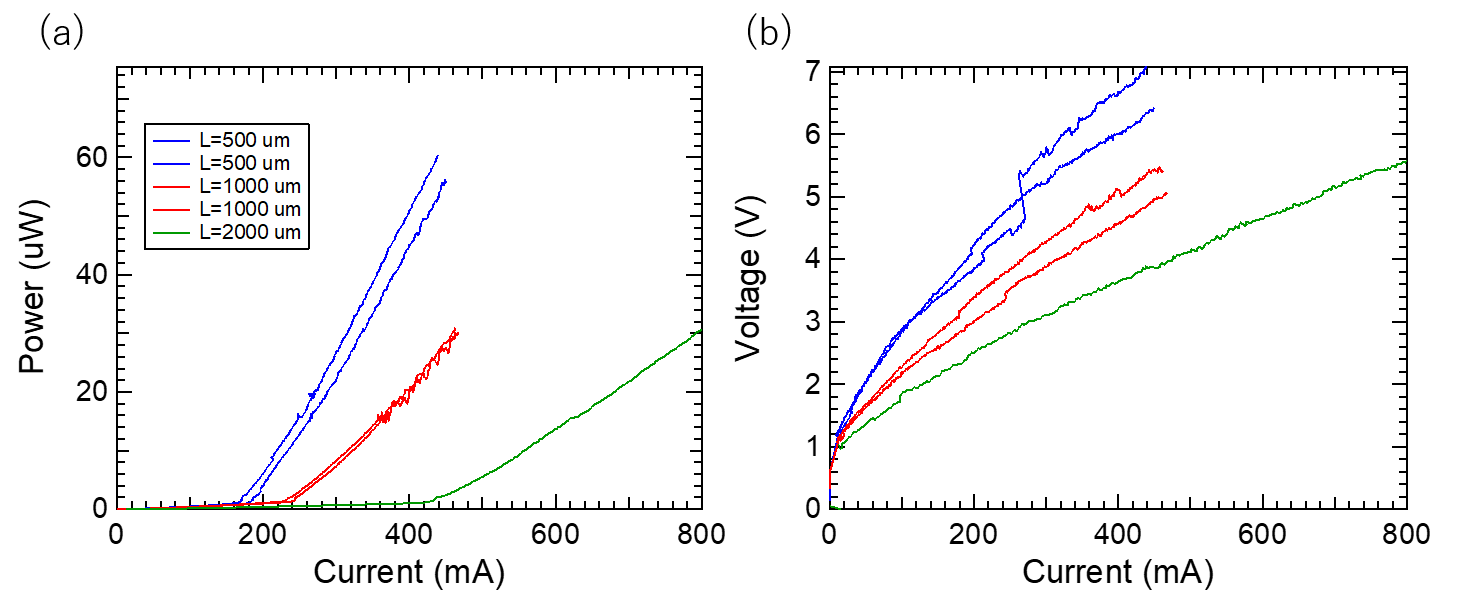
\includegraphics[width=12cm]{figure/fig_3_1_3QW_broadcontact_IL.png}
		\caption{3MQWのIL結果}
		\label{fig_3_1_3QW_broacdcontact_IL}
\end{figure}
次に様々なパッド幅に対して実験を行いフィッティングを行なったのでその結果を図\ref{fig_3_1_3QW_broadcontact_Ith}に示す。パッド幅が大きくなるにしたがって閾値電流が線形に増大することがわかる。一方すろーぷは。。。。。。
\begin{figure}[h]
	\centering
	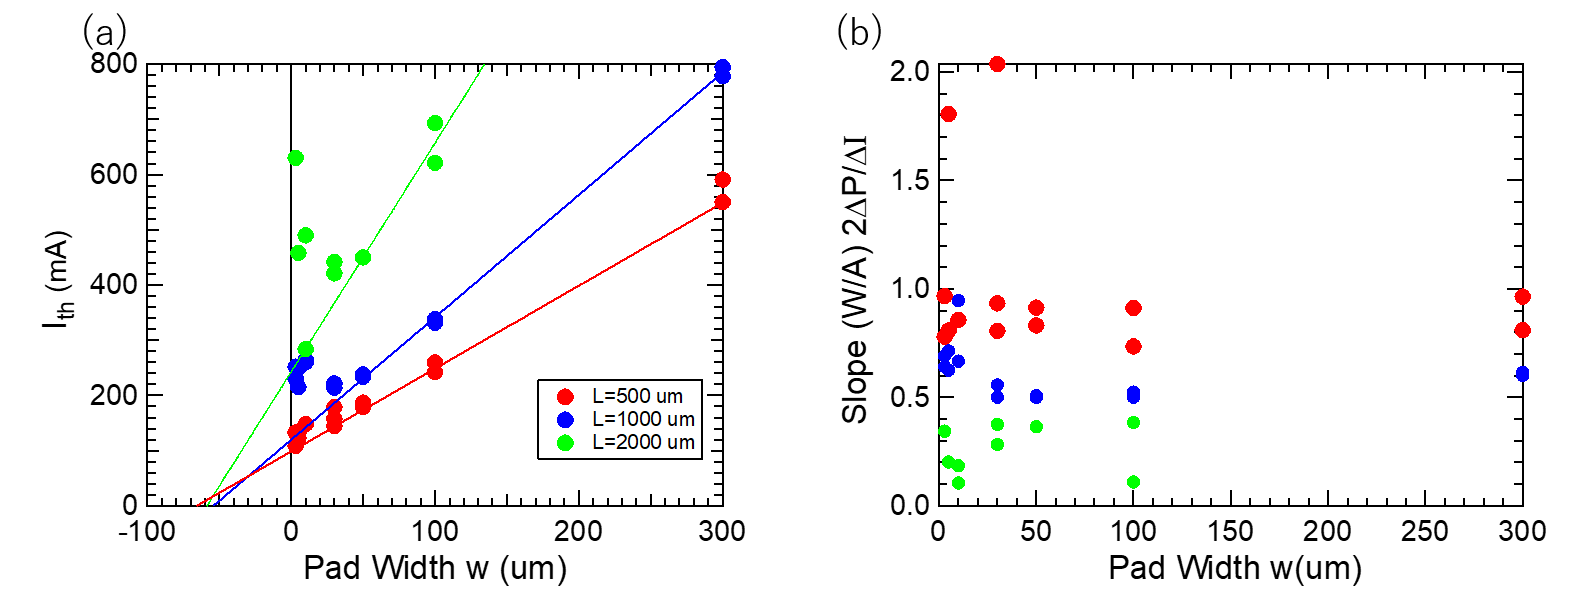
\includegraphics[width=15cm]{figure/fig_3_1_3QW_broadcontact_Ith.png}
		\caption{3MQWの閾値電流}
		\label{fig_3_1_3QW_broadcontact_Ith}
\end{figure}
\begin{comment}
閾値の表この表違うかも
\begin{table}[hbtp]
  \caption{閾値}
  \label{table:data_type}
  \centering
  \begin{tabular}{lcr}
    \hline
    共振器長  & 宣言  &  ビット幅  \\
    \hline \hline
    文字型  & char  & 8 \\
    整数型  & int   & 32 \\
    倍精度実数型  & double  & 64 \\
    倍々精度実数型  &  long double  &  96 \\
    \hline
  \end{tabular}
\end{table}
\end{comment}
\begin{comment}
\begin{figure}[h]
	\centering
	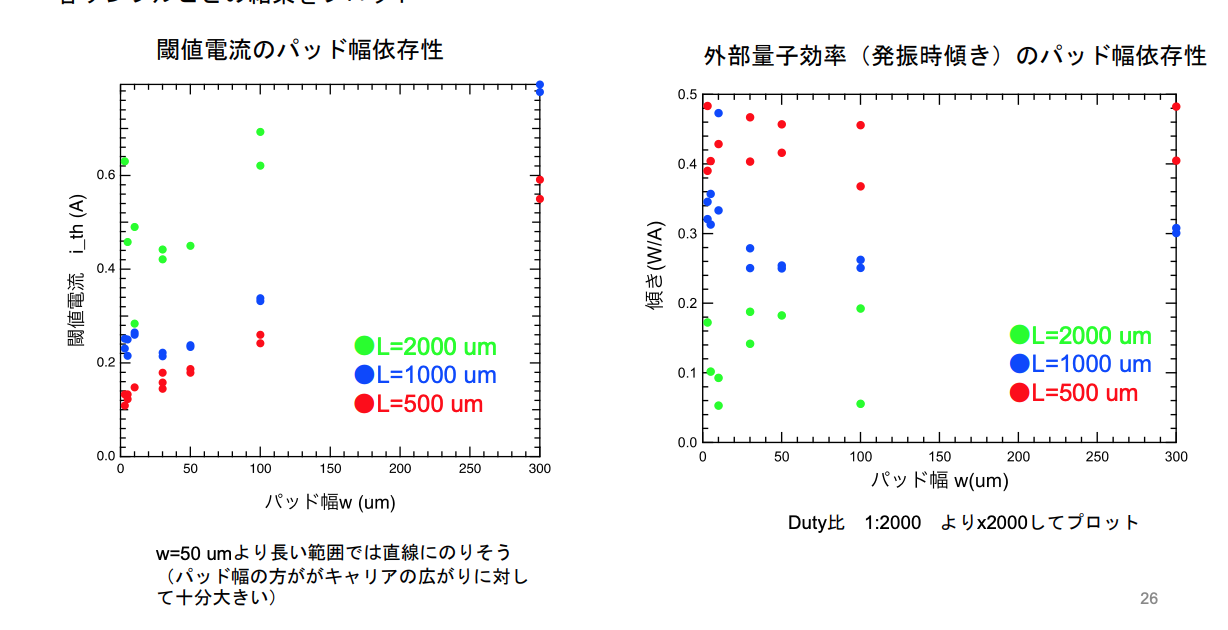
\includegraphics[width=10cm]{figure/fig_3_1_broad_i_th_3QW.png}
		\caption{3MQWの閾値電流}
		\label{fig_3_1_broad_i_th_3QW}
\end{figure}
\end{comment}
\begin{comment}
\begin{figure}[h]
	\centering
	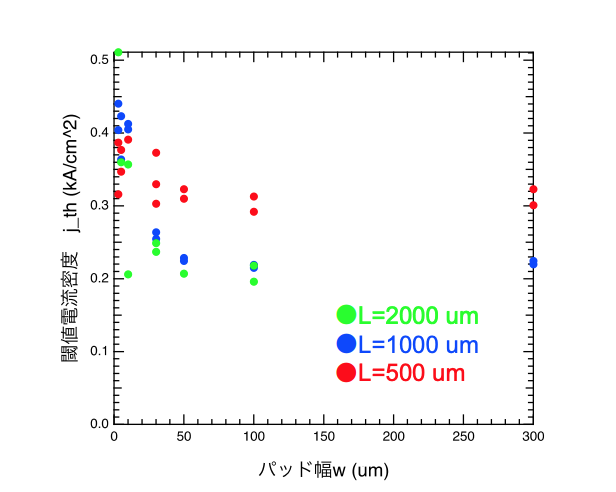
\includegraphics[width=15cm]{figure/fig_3_1_broad_j_th_3QW.png}
		\caption{3MQWの閾値電流密度のパッド幅依存性}
		\label{fig_3_1_broad_j_th_3QW}
\end{figure}
\end{comment}
\newpage
\subsection{10QW}%===============================
次に10周期量子井戸ブロードコンタクトレーザーについての結果を示す。ILカーブおよびIVカーブをw=50をだいひょうとしてしめす。いろわけは共振器ながさのちがいをあらわす。それぞれについてはっしんがかくにんできた。デューティー比は1対1000である。(2us 2ms周期)
\begin{figure}[h]
	\centering
	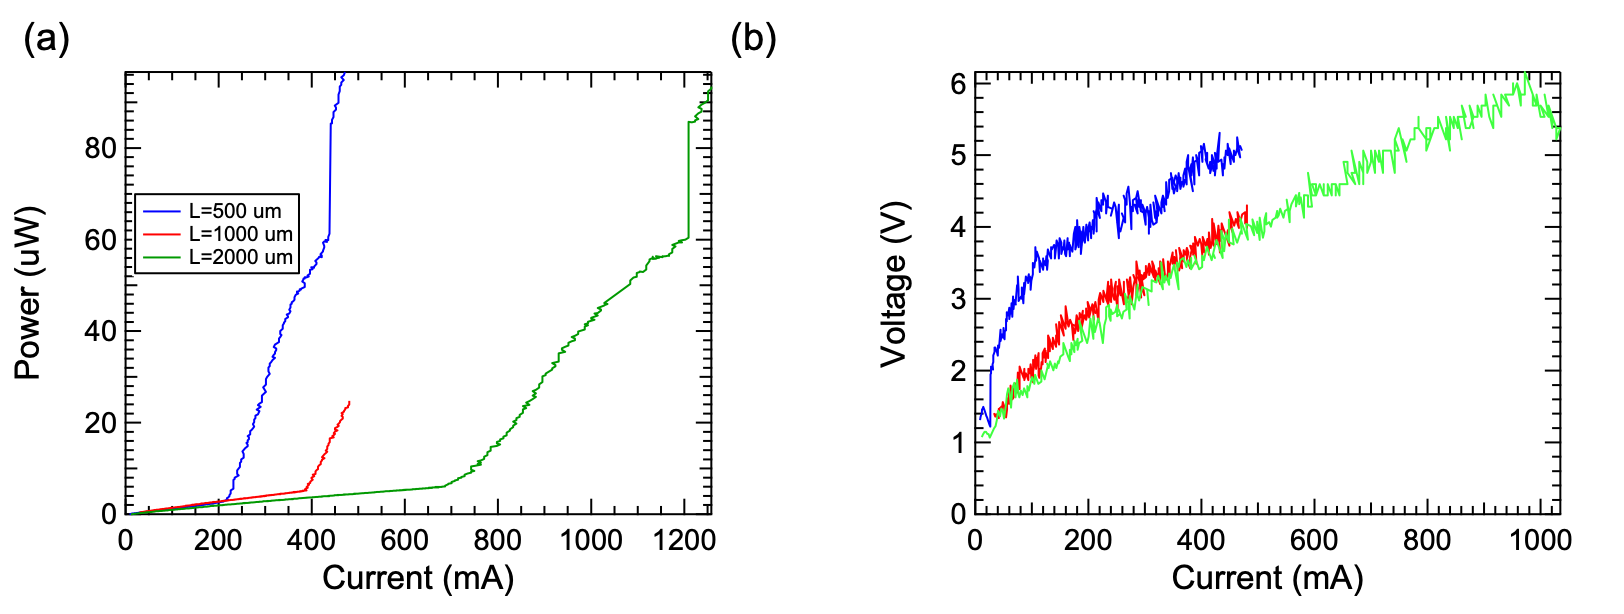
\includegraphics[width=15cm]{figure/fig_3_1_10QW_broadcontact_IL.png}
		\caption{10MQWのIL結果}
		\label{fig_3_1_10QW_broadcontact_IL}
\end{figure}
またILカーブの発振時の直線フィッティング結果から閾値電流Ithと傾きdP/dIをプロットした。dP/dIについてはdデューティー比を考慮してまた両端面からの発光を算出している。
\begin{figure}[h]
	\centering
	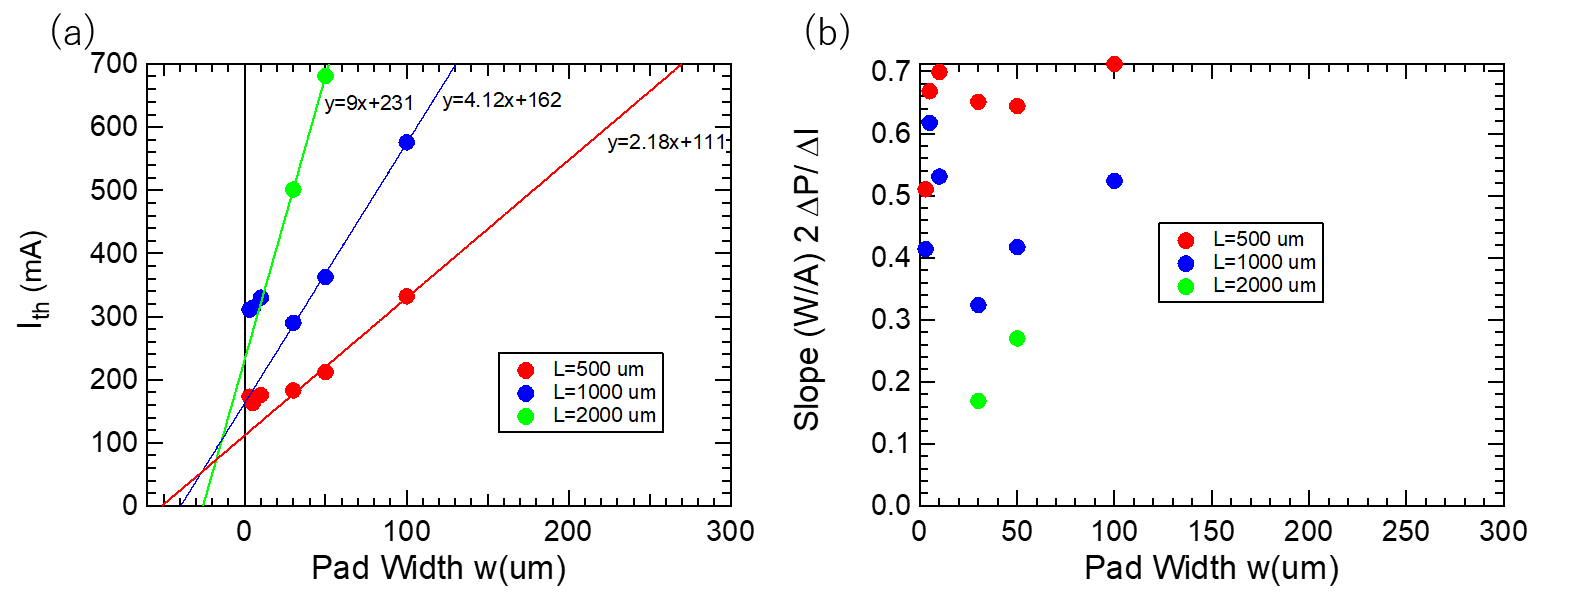
\includegraphics[width=15cm]{figure/fig_3_1_10QW_broadcontact_Ith.png}
		\caption{10MQWのIL結果}
		\label{fig_3_1_10QW_broadcontact_Ith}
\end{figure}


\newpage

\subsection{電流広がりに関する考察}%==================
レーザーの基本的な特性を知る上で閾値電流密度が大切なパラメータとなる。これを見積もるために先の節の結果からキャリアの広がりを見積もった。\\
 本体閾値電流電流は電流を流す面積に比例して大きくなるはずであるが図を見るとそうなっておらず赤ペンを持っている。そのx切片を含めたパッド幅を有効的な幅と考えて閾値電流密度を算出した。まずは有効パッド幅を見積もった。図\ref{fig_3_1_3QW_broadcontact_Ith}と図\ref{fig_3_1_10QW_broadcontact_Ith}それぞれの(a)においてIthが線形に増加する領域をフィッティングした。そのフィッティング関数のx切片の絶対値が実質的なパッド幅の増分である。その値を表に示した。
 
\begin{table}[hbtp]
  \caption{3QWブロードコンタクトレーザーの電流広がり}
  \label{table_3QW_broadcontact_w_eff}
  \centering
  \begin{tabular}{lcr}
    \hline
    共振器長L (um)  & パッド幅の増分(電流の広がり) w' (um)   \\
    \hline \hline
     500 & 65.8  \\
    1000  & 54.1 \\
    2000  & 58.7 \\ 
    \hline
  \end{tabular}
\end{table}

\begin{table}[hbtp]
  \caption{10QWブロードコンタクトレーザーの電流広がり}
  \label{table_10QW_broadcontact_w_eff}
  \centering
  \begin{tabular}{lcr}
    \hline
    共振器長L (um)  & パッド幅の増分(電流の広がり) w' (um)   \\
    \hline \hline
     500 & 51.1  \\
    1000  & 39.5 \\
    2000  & 25.7 \\ 
    \hline
  \end{tabular}
\end{table}
この表の値w'と閾値電流$I_{\rm{th}}$(mA)から式(\ref{eq:Jth}を用いて)閾値電流密度$J_{\rm{th}} \rm{(kA/cm^2)}$を算出した。
\begin{eqnarray}
J_{\rm{th}}=\dfrac{I_{\rm{th}}}{(w+w')L}
\label{eq:Jth}
\end{eqnarray}

その結果を示す。
\begin{figure}[h]
	\centering
	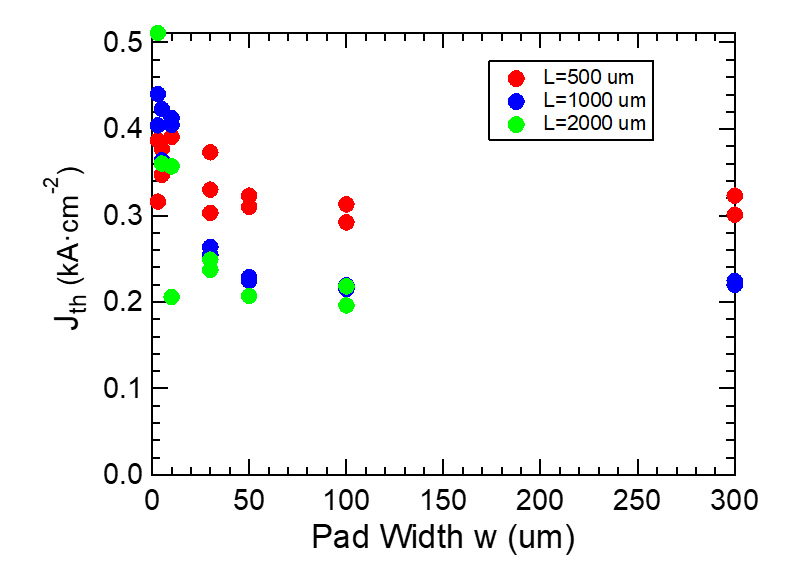
\includegraphics[width=10cm]{figure/fig_3_1_3QW_broadcontact_Jth.png}
		\caption{3MQWの閾値電流密度}
		\label{fig:fig_3_1_3QW_broadcontact_Ith}
\end{figure}
\begin{figure}[h]
	\centering
	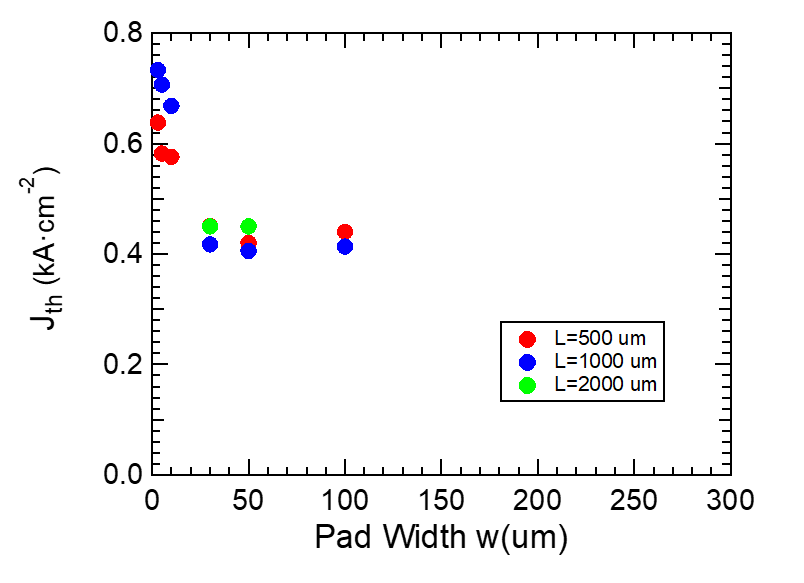
\includegraphics[width=10cm]{figure/fig_3_1_10QW_broadcontact_Jth.png}
		\caption{10MQWの閾値電流密度}
		\label{fig:fig_3_1_10QW_broadcontact_Ith}
\end{figure}
\newpage
\subsection{内部量子効率と吸収係数の計算}%=============
次にILカーブの発振時の傾きに相当する外部量子効率$\Delta P/\Delta I$から試料の内部量子効率および吸収係数を算出した。まずは外部量子効率の計算

\begin{figure}[htbp]
	\centering
	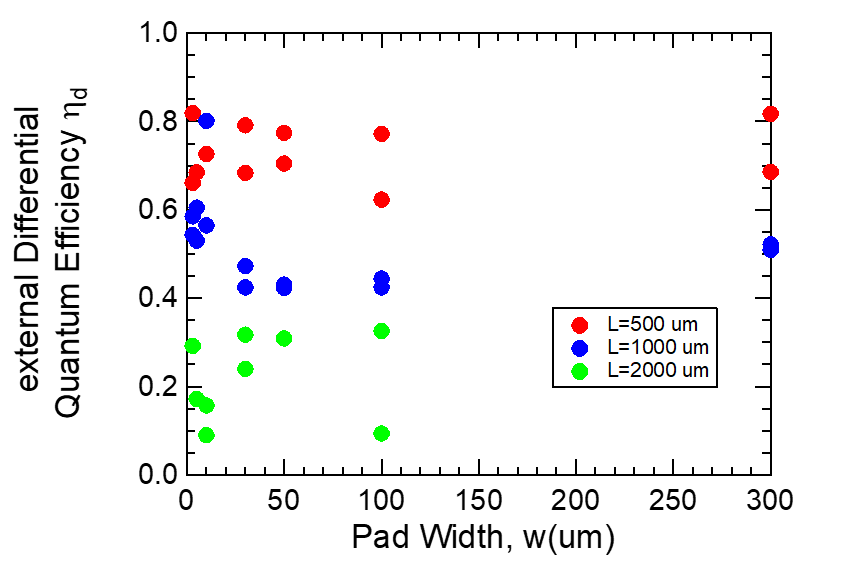
\includegraphics[width=10cm]{figure/fig_3_1_3QW_broadcontact_id.png}
	\caption{3QW外部量子効率}
	\label{fig:fig_3_1_3QW_broadcontact_id}
\end{figure}
次に内部量子効率を見積もった代表としてw=100umをプロットしている。
\begin{figure}[htbp]
	\centering
	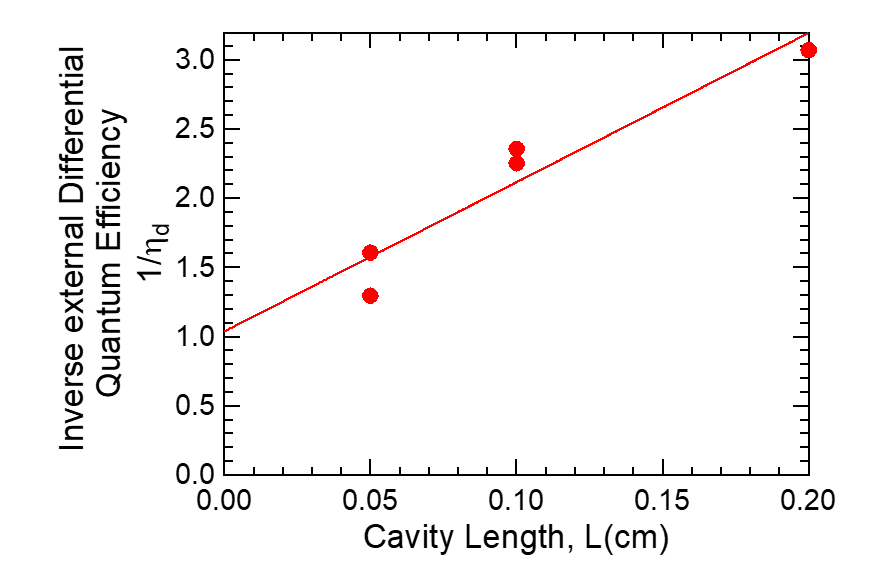
\includegraphics[width=10cm]{figure/fig_3_1_3QW_broadcontact_id_inverse.png}
	\caption{3QW外部量子効率の逆数}
	\label{fig:fig_3_1_3QW_broadcontact_id_inverse}
\end{figure}

同様の解析を10QWについても行った。
\begin{figure}[htbp]
	\centering
	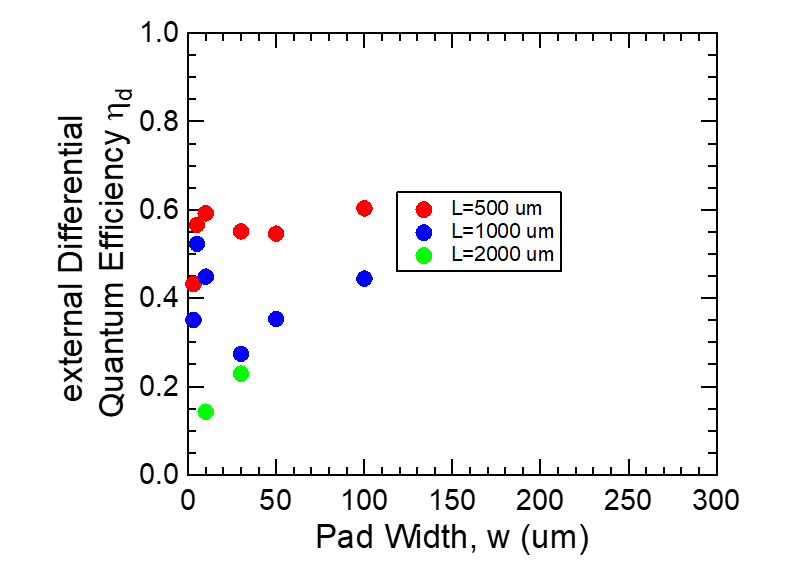
\includegraphics[width=10cm]{figure/fig_3_1_10QW_broadcontact_id.png}
	\caption{10QW外部量子効率の逆数}
	\label{fig:fig_3_1_10QW_broadcontact_id}
\end{figure}

\begin{figure}[htbp]
	\centering
	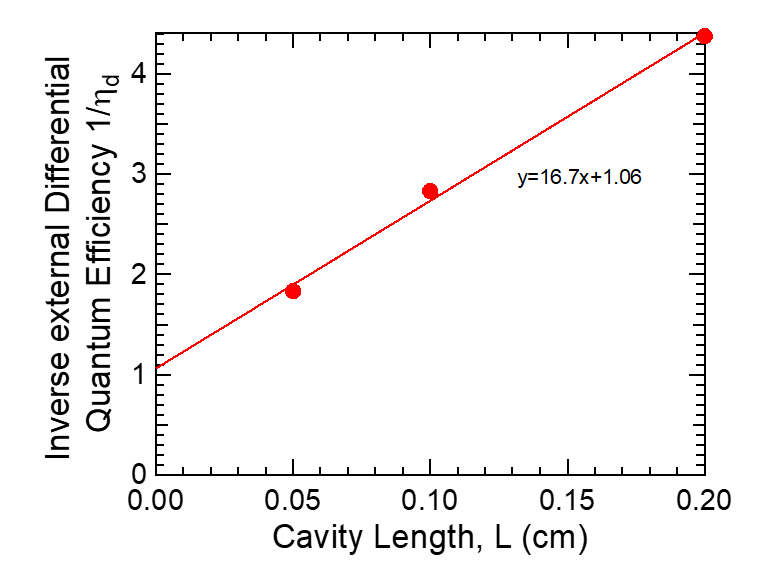
\includegraphics[width=10cm]{figure/fig_3_1_10QW_broadcontact_id_inverse.png}
	\caption{10QW外部量子効率の逆数}
	\label{fig:fig_3_1_10QW_broadcontact_id_inverse}
\end{figure}
\begin{comment}
\begin{figure}[h]
	\centering
	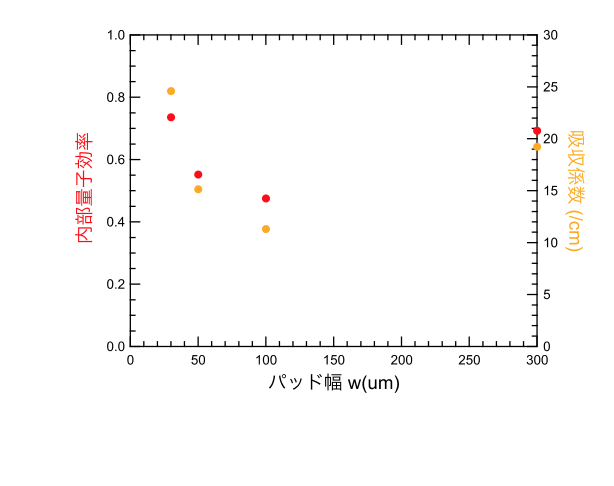
\includegraphics[width=10cm]{figure/fig_3_1_eff_in_3QW.png}
		\caption{3MQWのIL結果}
		\label{fig_3_1_IL_broad_i_th_3QW}
\end{figure}
\end{comment}

\newpage
\newpage
\newpage
\subsection{本節のまとめ}
ここまででブロードコンタクトレーザーを評価することにより物性パラメータを算出することができた。これらの値はレート方程式にもあらわれ?計算に用いることができる。
\section{リッジ導波路型レーザーに関する実験結果}%===================
次に実リッジ導波路型レーザーに関する実験結果を示す。リッジ導波路型レーザーはリッジを作っており、横方向の光閉じ込めを行なっている。
\subsection{定常電流の結果}
リッジ導波路型レーザーに関して電流注入利得スイッチング実験を行った。その時の光出力の時間はけいを示す。
励起時間は
\subsection{利得スイッチング動作の結果}
\subsubsection{3QW}%===============================
L=100,200,300

\subsubsection{10QW}%==============================
L=300,400,500
\begin{figure}[h]
	\centering
	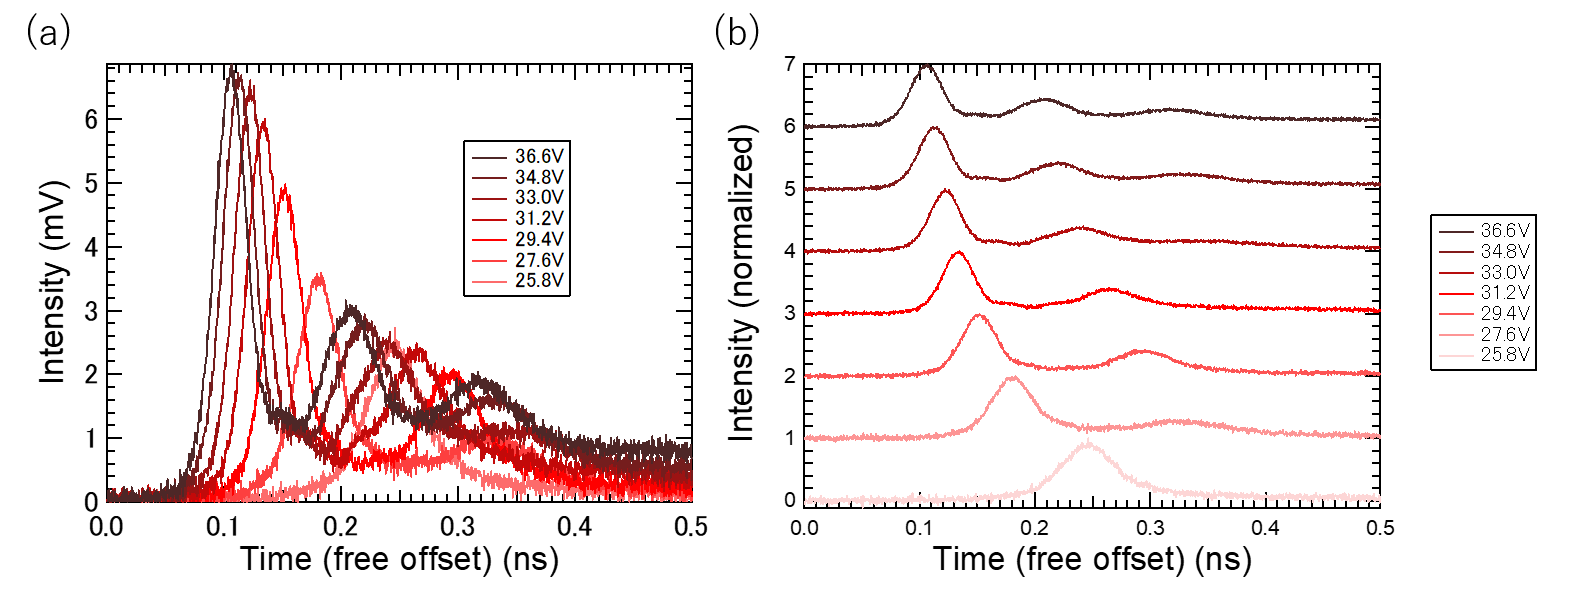
\includegraphics[width=10cm]{figure/fig_3_2_10QW_ridge_L300_GS.png}
		\caption{10MQW L=300um の利得スイッチング光パルスの時間波形}
		\label{fig:fig_3_2_10QW_ridge_L400_GS}
\end{figure}

\begin{figure}[h]
	\centering
	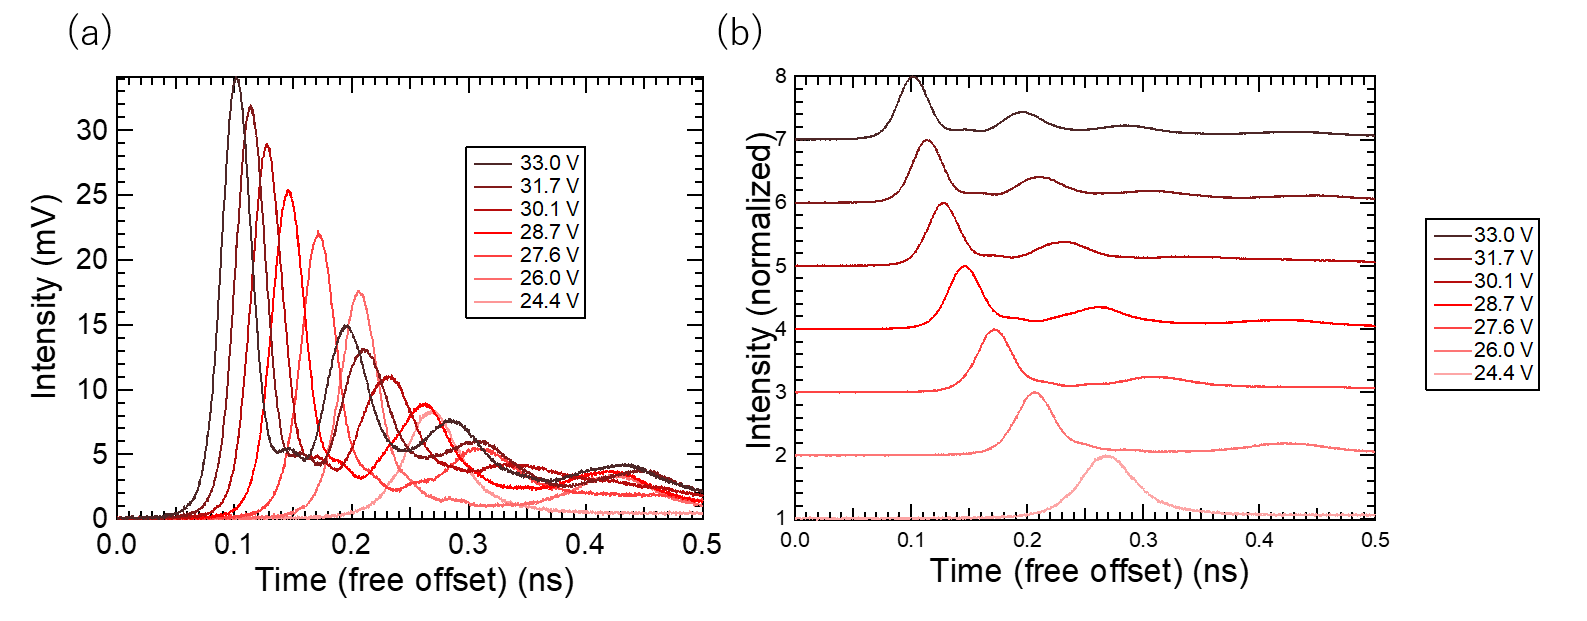
\includegraphics[width=10cm]{figure/fig_3_2_10QW_ridge_L400_GS.png}
		\caption{10MQW L=400um の利得スイッチング光パルスの時間波形}
		\label{fig:fig_3_2_10QW_ridge_L400_GS}
\end{figure}
\begin{figure}[h]
	\centering
	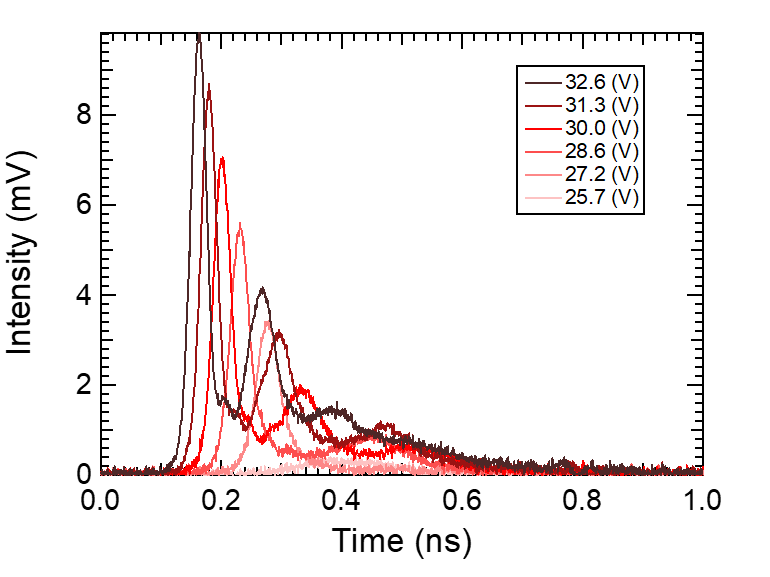
\includegraphics[width=10cm]{figure/fig_3_2_10QW_ridge_L500_GS.png}
		\caption{10MQW L=500um の利得スイッチング光パルスの時間波形}
		\label{fig:fig_3_2_10QW_ridge_L500_GS}
\end{figure}
\subsection{結果の比較}%===========================
FWHM でコンボリューションした物をまとめた。
\begin{figure}[h]
	\centering
	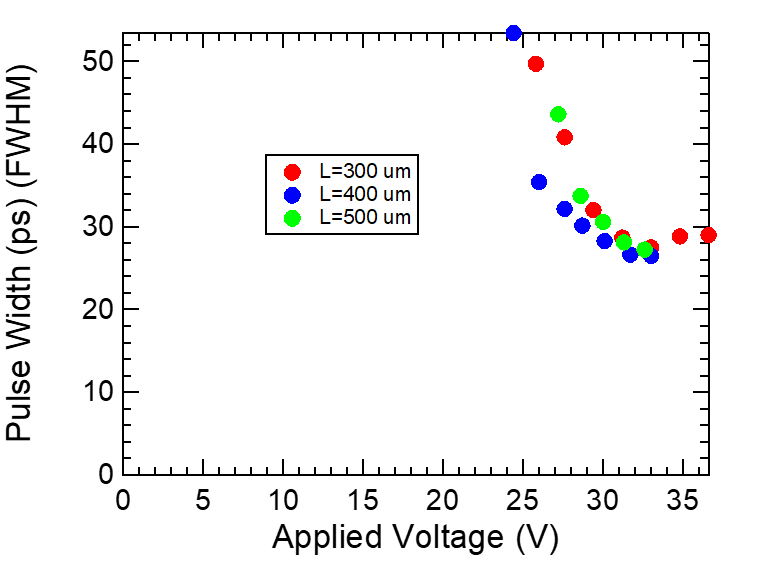
\includegraphics[width=10cm]{figure/fig_3_2_10QW_ridge_GS_FWHM.png}
		\caption{10MQW 利得スイッチングパルスのパルス幅}
		\label{fig:fig_3_2_10QW_ridge_GS_FWHM}
\end{figure}
\subsection{付録かな??コンボリュージョンの説明,電気パルスの確認}%==============

\begin{figure}[h]
	\centering
	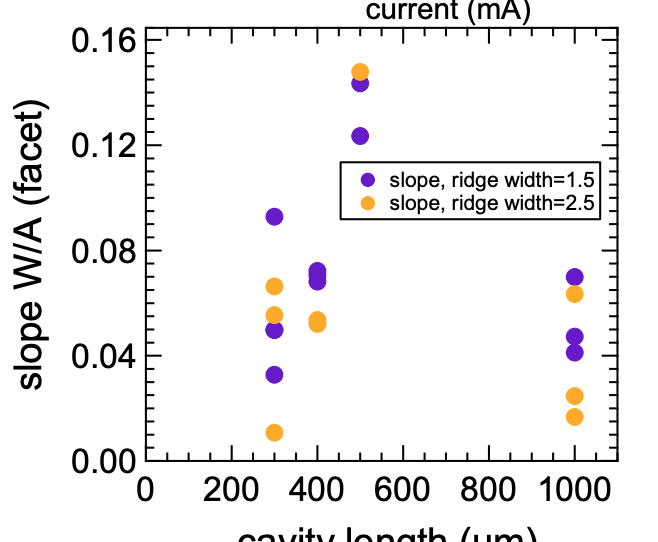
\includegraphics[width=10cm]{figure/fig_3_1_broad_slope_10QW.png}
		\caption{10MQWのスロープ}
		\label{fig_3_1_IL_broad_slope}
\end{figure}

\begin{figure}[h]
	\centering
	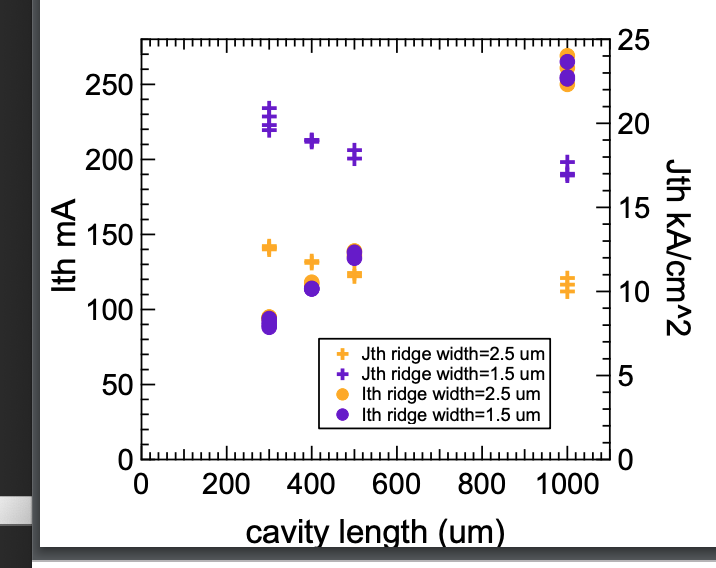
\includegraphics[width=10cm]{figure/fig_3_1_broad_i_th_10QW.png}
		\caption{10MQWの閾値電流}
		\label{fig_3_1_broad_i_th_3QW}
\end{figure}


\begin{figure}[h]
	\centering
	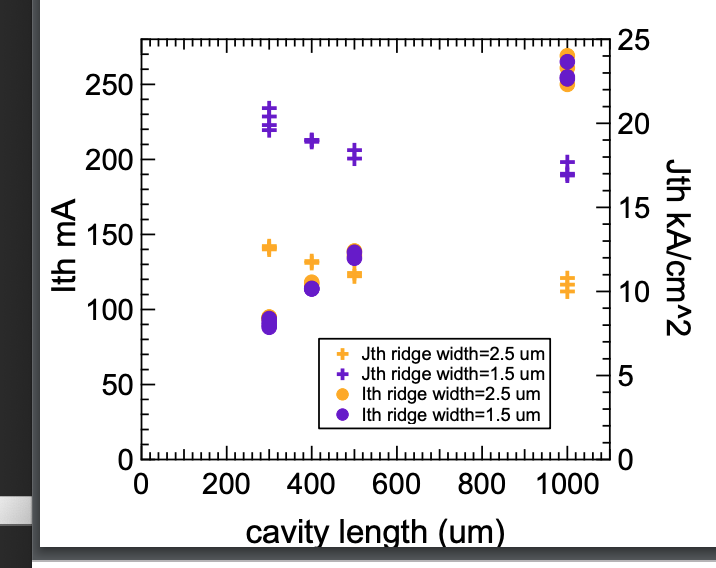
\includegraphics[width=10cm]{figure/fig_3_1_broad_i_th_10QW.png}
		\caption{10MQWの閾値電流密度のパッド幅依存性}
		\label{fig_3_1_broad_j_th_10QW}
\end{figure}
